\documentclass[a4paper]{article}

\usepackage{fontspec}
\usepackage{polyglossia}

\setmainlanguage{russian}
\setotherlanguages{english}

% download "Linux Libertine" fonts:
% http://www.linuxlibertine.org/index.php?id=91&L=1
\setmainfont{Linux Libertine O} % or Helvetica, Arial, Cambria
% why do we need \newfontfamily:
% http://tex.stackexchange.com/questions/91507/
\newfontfamily{\cyrillicfonttt}{Linux Libertine O}

\usepackage{amsmath} % Математические окружения AMS
\usepackage{amsfonts} % Шрифты AMS
\usepackage{amssymb} % Символы AMS
\usepackage{mathtext} % Русские буквы в фомулах
\usepackage{graphicx} % Вставить pdf- или png-файлы

\usepackage{color}
\usepackage{bbold}

\usepackage{booktabs}

\usepackage{mathrsfs} % Красивый шрифт

\usepackage{longtable}  % Длинные таблицы
\usepackage{multirow} % Слияние строкв таблице

\usepackage{indentfirst} % Отступ в первом абзаце.
\usepackage{tikz}

\newcommand*{\hm}[1]{#1\nobreak\discretionary{}%
            {\hbox{$\mathsurround=0pt #1$}}{}}

\usepackage{verbatim}

\DeclareMathOperator{\sgn}{\mathop{sgn}}
\DeclareMathOperator{\card}{\mathop{card}}

\usepackage{enumitem}


\usepackage{fancyhdr}
\usepackage[margin=1in]{geometry}


\AddEnumerateCounter{\asbuk}{\russian@alph}{щ} % для списков с русскими буквами
\setlist[enumerate, 2]{label=\asbuk*),ref=\asbuk*}


\pagestyle{fancy} \makeatletter \fancyhead[L]{\footnotesize ICEF, 2016/17, «Mathematics for Economists»}

\makeatletter
\newcommand*{\rom}[1]{\expandafter\@slowromancap\romannumeral #1@}
\makeatother

\usepackage{wrapfig}

 \begin{document}
 \begin{center}
 {\Large{Конспект лекции 13.12.16}}
 \end{center}
  \begin{center}
 {\large{Живайкина Александра}}
 \end{center}
 \par {\bf\underline{Упражнение 1.}} Взять стохастический интеграл в непрерывном времени:

 $$\int\limits_{0}^{t}W_udW_u$$

 Это первый и единственный стохастический интеграл, который мы будем брать по определению, так как взятие интеграла по определению всегда наиболее долгий и трудоемкий способ решения.\\

 Разделим интервал от 0 до t на n частей, а затем устремим $n \rightarrow \infty$.

 \begin{figure}[h]
 \center{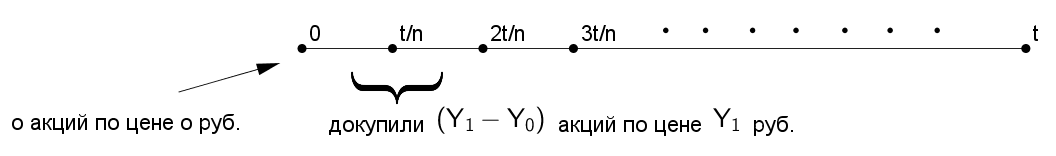
\includegraphics[width=1\linewidth]{05_graph.png}}
 \label{image}
 \end{figure}

 Для удобства переобозначим:

 \begin{equation*}
 \begin{aligned}
 Y_1 &= W_{\frac{t}{n}}\\
 Y_2 &= W_{\frac{2t}{n}}\\
 &\vdots\\
 Y_{n-1} &= W_{\frac{(n-1)t}{n}}\\
 Y_n &= W_t
 \end{aligned}
 \end{equation*}

 Чтобы решить поставленную задачу, сначала необходимо найти дискретную версию $(I_n)$ исходного стохастического интеграла, а потом вычислить предел $I_n$ в смысле $L^2$ при $n \rightarrow \infty$:

 $$I_n \xrightarrow{L^2} I$$

 $\bullet$ Дискретная версия интеграла записывается следующим образом:

 $$I_n = -0 + Y_n \cdot Y_n - \left(Y_1-Y_0\right)\cdot Y_1-\left(Y_2-Y_1\right)\cdot Y_2-\cdots-\left(Y_n-Y_{n-1}\right)\cdot Y_n$$

 \begin{flushleft}
 где\\
 0 --- изначальное богатство\\
 $Y_n \cdot Y_n$ --- конечное богатство\\
 $\left(Y_1-Y_0\right)\cdot Y_1-\left(Y_2-Y_1\right)\cdot Y_2-\cdots$ --- затраты на покупку дополнительных акций
 \end{flushleft}

 Таким образом, получаем, что:
 \begin{equation}\label{eq:I_n}
 I_n=Y^{2}_{n}-\sum_{i=1}^{n}Y_i\cdot\left(Y_i-Y_{i-1}\right)
 \end{equation}

 Однако у $I_n$ считать предел не удобно, так как $Y_i$ и $Y_i-Y_{i-1}$ зависимы. Лучше сначала вычислить предел величины $J_n$, у которой приращения броуновского движения не зависимы, а потом перейти от $J_n$ к $I_n$.

 $J_n$ записывается следующим образом:

 \begin{equation}\label{eq:J_n}
   J_n=\sum_{i=1}^{n}\left(Y_i-Y_{i-1}\right)^2
   \end{equation}

 \newpage
 $\bullet$ Возьмем предел величины $J_n$ в смысле $L^2$ при $n \rightarrow \infty$.\\

 Обратим внимание, что $Y_i-Y_{i-1}$ показывает, насколько броуновское движение изменилось за данный промежуток времени $\frac{t}{n}$. Все эти интервалы времени не пересекаются, поэтому разницы броуновского движения не зависимы.\\

 Заметим, что $Y_i-Y_{i-1}$ имеет нормальный закон распределения с параметрами:

  $$Y_i-Y_{i-1}\sim \mathcal{N}\left(0,\frac{t}{n}\right)$$

 Математическое ожидание и дисперсия $J_n$ равны:

  $$E(J_n)=E\left(\sum\left(Y_i-Y_{i-1}\right)^2\right)=\sum E\left(\left(Y_i-Y_{i-1}\right)^2\right)=n\cdot Var\left(Y_i-Y_{i-1}\right)^2=n\cdot\frac{t}{n}=t$$
  \begin{multline*}
  Var(J_n)=n\cdot Var\left(\left(Y_i-Y_{i-1}\right)^2\right)=\langle\text{сделаем единичную дисперсию}\rangle=n\cdot Var\left(\left(\frac{Y_i-Y_{i-1}}{\sqrt{\frac{t}{n}}}\right)^2\cdot\frac{t}{n}\right)=\\
  =n\cdot\left(\frac{t}{n}\right)^2\cdot Var\left(\left(\mathcal{N}\left(0;1\right)\right)^2\right)=\frac{t^2}{n}\cdot\chi^2(1)=\frac{t^2}{n}\cdot2\xrightarrow{n\rightarrow\infty}0
  \end{multline*}


 Таким образом, при $n \rightarrow \infty$ последовательность $J_n \xrightarrow{L^2} t.$\\

 $\bullet$ Выразим $I_n$ через $J_n$.\\

 Раскроем скобки в \eqref{eq:I_n} и \eqref{eq:J_n} уравнениях:

 $$I_n=Y^{2}_{n}-\sum_{i=1}^{n}Y^{2}_{i}+\sum_{i=1}^{n}Y_i\cdot Y_{i-1}$$

 $$J_n=\sum_{i=1}^{n}Y^{2}_{i}+\sum_{i=1}^{n}Y^{2}_{i-1}-2\sum_{i=1}^{n}Y_i\cdot Y_{i-1}=2\sum_{i=1}^{n}Y^{2}_{i}-2\sum_{i=1}^{n}Y_i\cdot Y_{i-1}-Y^{2}_{n}$$

 Таким образом, связь между $I_n$ и $J_n$ равна:

 $$J_n=-2I_n+Y^{2}_{n}$$

 Сделаем обратную замену:
 \begin{equation}\label{eq:connection}
 J_n=-2I_n+W^{2}_{t}
 \end{equation}

 $\bullet$ Устремляем левую и правую часть уравнения \eqref{eq:connection} в $L^2$. \\

 Мы знаем, что $J_n \xrightarrow{L^2} t$, $I_n \xrightarrow{L^2} I$, а $W^{2}_{t}$ от $n$ не зависит. Следовательно, получаем:

 $$t=-2I+W^{2}_{t}$$

 $$I=\frac{W^{2}_{t}-t}{2}$$

 Таким образом, стохастический интеграл в непрерывном времени имеет вид:

 \begin{equation*}
  \fbox{$I=\int\limits_{0}^{t}W_udW_u=\frac{W^{2}_{t}-t}{2}$}
  \end{equation*}

 \begin{wrapfigure}{l}{0.1\linewidth}
     
\includegraphics[width=\linewidth]{05_sign.jpg}
 \end{wrapfigure}

 Важно помнить, что из-за случайности стохастические интегралы \underline{\bf{нельзя}} брать как обычные интегралы.

 $$\int\limits_{0}^{t}W_udW_u=\frac{W^{2}_{t}-W^{2}_{0}}{2}=\frac{W^{2}_{t}}{2} \text{--- это неправильно.}$$

 \vspace{1pt}

 \begin{center}
 \Large\it{Свойства стохастического интеграла}
 \end{center}

 Введем несколько \underline{условий}, которые всегда будем предполагать в дальнейшем:\\

 1) Процесс $(X_t)$ адаптирован к фильтрации $(\mathcal{F}_t)$\\

 2) $\int\limits_{0}^{t}E(X^{2}_{u}du)<\infty$\\

 Перейдем к \underline{свойствам}:

 \begin{enumerate}[label={\theenumi)}]
 \item $\int\limits_{0}^{t}\left(aX_u+bY_u\right)dW_u=a\int\limits_{0}^{t}X_udW_u+b\int\limits_{0}^{t}Y_udW_u$\\
 \item
 $\int\limits_{a}^{b}X_udW_u+\int\limits_{b}^{c}X_udW_u=\int\limits_{a}^{c}X_udW_u$\\
 \item
 $I_t=\int\limits_{0}^{t}X_udW_u$ --- это мартингал\\

 Следовательно:\\

 $E(I_{t+\delta}|\mathcal{F}_t)=I_t \Rightarrow E(I_{t+\delta})=I_t$\\

 Например, если $t=0, \delta=t$, то

 $E(I_t)=E(I_0)=0 \Rightarrow$ В любой момент времени математическое ожидание одинаково\\

 \item\label{cov}
 $cov\left(\int\limits_{o}^{t}X_udW_u,\int\limits_{o}^{t}Y_udW_u\right)=\int\limits_{0}^{t}E\left(X_u\cdot Y_u\right)du$ --- ковариация стохастических интегралов равна обычному интегралу\\

 В частном случае: $Var\left(\int\limits_{0}^{t}X_udW_u\right)=\int\limits_{0}^{t}E\left(X^{2}_{u}\right)du$\\

 \item
 \underline{\bf \large Лемма Ито}\\

 Версии по сложности:\\
 $\rightarrow$ лайт-версия\\
 $\rightarrow$ рабочая версия\\
 $\rightarrow$ версия <<попонтоваться>>\\

 Формы записи:\\
 $\rightarrow$ полная\\
 $\rightarrow$ сокращенная

 \end{enumerate}

 \newpage

 \par {\bf\underline{Определение.}} {\it\bf Сокращенная форма записи интегралов} \\

 Процесс вида: $$R_t=R_0+\int\limits_{0}^{t}X_udW_u+\int\limits_{0}^{t}Y_udu, \text{где $R_0$ --- это константа,}$$

 называется процессом Ито и кратко записывается:
 $$dR_t=X_tdW_t+Y_tdt$$

 Сокращенную форму записи никак нельзя интерпретировать, так как $dR_t, dW_t$ сами по себе не существуют.\\

 Например, в математике из условной формы записи $x^2=0(x)$ и $x^3=0(x)$ \underline{\bf не следует} то, что $x^2=x^3$\\

 \par {\bf\underline{Упражнение 2.}} Дана краткая форма записи: $dX_t=W_tdW_t+7dt$\\

 Записать процесс в полной форме.\\

 Решение: $X_t=X_0+\int\limits_{0}^{t}W_udW_u+\int\limits_{0}^{t}7du$\\

 \par {\bf\underline{Упражнение 3.}} Переформулировать свойство \ref{cov} (про ковариации) в краткой записи.\\

 Решение: $cov\left(X_tdW_t, Y_tdW_t\right)=E(X_t,Y_t)dt$\\

 {\large\it\bf \underline{Лемма Ито (лайт-версия)} \\

 $\bullet$ в краткой форме записи}\\

 Если $Y_u=f(W_u,u)$ и $f^{''}_{ww}, f^{'}_{u}$ --- непрерывные функции, то \fbox{$dY_t=f^{'}_{w}dW_t+f^{'}_{t}dt+\frac{1}{2}f^{''}_{ww}dt$}\\

 {\large\it\bf $\bullet$ в полной форме записи}\\

 \fbox{$Y_t=Y_0+\int\limits_{0}^{t}f^{'}_{w}(W_u,u)dW_u+\int\limits_{0}^{t}f^{'}_{u}(W_u,u)du+\frac{1}{2}\int\limits_{0}^{t}f^{''}_{ww}(W_u,u)du$}\\ \\

 \par {\bf\underline{Упражнение 4.}} Для каждого пункта найти $dY_t$ и выписать утверждение в полной форме.

 \begin{enumerate}[label={\alph*)}]
 \item $Y_t=W^{2}_{t}$\\

 Решение: $dY_t=2W_tdW_t+0dt+\frac{1}{2}\cdot 2dt=2W_tdW_t+dt$\\

 $Y_t=Y_0+2\int\limits_{0}^{t}W_udW_u+\int\limits_{0}^{t}du$\\

 $W^{2}_{t}=0+2\int\limits_{0}^{t}W_udW_u+t \Rightarrow \int\limits_{0}^{t}W_udW_u=\frac{W^{2}_{t}-t}{2}$

 \item $Y_t=W_t\cdot t$\\

 Решение: $dY_t=tdW_t+W_tdt$\\

 $Y_t=Y_0+\int\limits_{0}^{t}udW_u+\int\limits_{0}^{t}W_udu$\\

 $W_t\cdot t=\int\limits_{0}^{t}udW_u+\int\limits_{0}^{t}W_udu$

 \item\label{c} $Y_t=cos(W_t)-t$\\

 Решение: $dY_t=-\sin(W_t)dW_t-dt-\frac{1}{2}\cos(W_t)dt$\\

 $Y_t=Y_0-\int\limits_{0}^{t}\sin(W_u)dW_u-\int\limits_{0}^{t}du-\frac{1}{2}\int\limits_{0}^{t}\cos(W_u)du$\\

 $\cos(W_t)-t=\cos(W_0)-\int\limits_{0}^{t}\sin(W_u)dW_u-t-\frac{1}{2}\int\limits_{0}^{t}\cos(W_u)du=1-\int\limits_{0}^{t}\sin(W_u)dW_u-t-\frac{1}{2}\int\limits_{0}^{t}\cos(W_u)du$\\

 \item\label{d} $Y_t=W^{4}_{t}$\\

 $dY_t=4W^{3}_{t}dW_t+6W^{2}_{t}dt$\\

 $Y_t=W^{4}_{t}=4\int\limits_{0}^{t}W^{3}_{u}dW_u+6\int\limits_{0}^{t}W^{2}_{u}du$\\

 \item\label{e} $Y_t=t^2\cdot W^{3}_{t}$\\

 $dY_t=3t^2\cdot W^{2}_{t}dW_t+2tW^{3}_tdt+3t^2W_tdt$\\

 $Y_t=t^2\cdot W^{3}_{t}=3\int\limits_{0}^{t}u^2\cdot W^{2}_{u}dW_u+2\int\limits_{0}^{t}uW^{3}_{u}du+3\int\limits_{0}^{t}u^2\cdot W_{u}du$
 \end{enumerate}

 \ref{c}, \ref{d}, \ref{e} --- решить дома\\

{\large\it {\bf\underline{Способ запомнить} формулировку леммы Ито в краткой условной записи} \\
(не доказательство и не буквальное равенство)} \\

Необходимо разложить в ряд Тейлора до второго порядка и упростить по принципу:

\begin{align*}
dW\cdot dW = dt & \Rightarrow \sum_{i=1}^{n}(Y_i-Y_{i-1})^2 \xrightarrow{L^2} t, \text{при } n\rightarrow\infty\\
dt\cdot dt = 0 & \Rightarrow \sum_{i=1}^{n}(\Delta t)^2 \xrightarrow{L^2} 0, \text{при } n\rightarrow\infty\\
dt\cdot dW = 0 & \Rightarrow \sum_{i=1}^{n}\Delta t(Y_i-Y_{i-1}) \xrightarrow{L^2} 0, \text{при } n\rightarrow\infty
\end{align*}

 {\large\it\bf \underline{Рабочая лемма Ито}}\\

 Если $dX_t=A_tdW_t+B_tdt$ и $Y_t=f(X_t,t)$ и $f^{''}_{xx}, f^{'}_{t}$ --- непрерывные функции, то:\\

 $dY_t=f^{'}_{x}dX_t+f^{'}_tdt+\frac{1}{2}\left(f^{''}_{xx}dX\cdot dX+f^{''}_{xt}dX\cdot dt+f^{''}_{tt}dt\cdot dt\right)=\fbox{$f^{'}_xdX+f^{'}_tdt+\frac{1}{2}f^{''}_{xx}\cdot A^{2}_{t}dt$}$\\

\par {\bf\underline{Упражнение 5.}} Найти $dY_t$ и восстановить полную форму записи.

\begin{enumerate}[label={\alph*)}]
\item $dX_t=W^{2}_{t}\cdot dW_t+W_t\cdot dt$\\

$Y_t=X^{2}_{t}\cdot t \Rightarrow Y_0=0$\\

Решение: $dY_t=2X_t\cdot tdX+X^{2}_{t}dt+\frac{1}{2}\cdot 2t\cdot W^{4}_{t}dt=2X_t\cdot t\cdot (W^{2}_{t}\cdot dW_t+W_t\cdot dt)+X^{2}_{t}dt+t\cdot W^{4}_{t}dt$\\

$Y_t=2\int\limits_{0}^{t}X_u\cdot u\cdot W^{2}_{u}dW_{u}+2\int\limits_{0}^{t}X_u\cdot u\cdot W_udu+\int\limits_{0}^{t}X^{2}_{u}du+\int\limits_{0}^{t}u\cdot W^{4}_{u}du$\\

\item $dX_t=cos(W_t)dW_t+sin(W_t)dt$\\

$Y_t=X^{2}_{t} \Rightarrow Y_o=X^{2}_{0}$\\

Решение: $dY_t=2X_tdX+0+\frac{1}{2}\cdot 2\cdot cos^2(W_t)dt=2X_t\cdot (cos(W_t)dW_t+sin(W_t)dt)+cos^2(W_t)dt$\\

$Y_t=X^{2}_{0}+2\int\limits_{0}^{t}X_u\cdot cos(W_u)dW_u+2\int\limits_{0}^{t}X_u\cdot sin(W_u)du+\int\limits_{0}^{t}cos^2(W_u)du$

\end{enumerate}

\par {\bf\underline{Упражнение 6.}} В модели Блэка-Шоулза предполагается, что цена акции $S_t$ подчиняется стохастическому дифференциальному уравнению:

$$dS_t=\mu S_tdt+\delta S_tdW_t$$
$$Y_t=\ln S_t$$

\begin{enumerate}[label={\alph*)}]
\item Найти $dY_t$ и восстановить полную форму записи.\\

Решение:
\begin{multline*}
dY_t=\frac{1}{S_t}dS_t+0+\frac{1}{2}\cdot \left(-\frac{1}{S^{2}_{t}}\right)\cdot (dS_t)^2=\frac{1}{S_t}dS_t-\frac{1}{2}\cdot \frac{1}{S^{2}_{t}}\cdot \delta^2\cdot S^{2}_{t}dt=\\
=\frac{1}{S_t}\cdot(\mu S_tdt+\delta S_tdW_t)-\frac{1}{2}\cdot \frac{1}{S^{2}_{t}}\cdot \delta^2\cdot S^{2}_{t}dt=\mu dt+\delta dW_t-\frac{1}{2}\delta^2dt
\end{multline*}

$Y_t=Y_0+\mu \int\limits_{0}^{t}du+\delta \int\limits_{0}^{t}dW_u-\frac{1}{2}\delta^2\int\limits_{0}^{t}du=Y_0+\mu t+\delta W_t-\frac{\delta^2}{2}t=Y_0+\delta W_t+\left(\mu-\frac{\delta^2}{2}\right)t$\\

\item Найти $S_t$ в явном виде.\\

Решение:\\

$\ln S_t=\ln S_0+\delta W_t+\left(\mu-\frac{\delta^2}{2}\right)t$\\

$S_t=S_0+\exp^{\delta W_t+\left(\mu-\frac{\delta^2}{2}\right)t}$

\end{enumerate}

\par {\bf\underline{Упражнение 7.}} №5 с пересдачи 2015 года.

\begin{equation*}
	\left\{
		\begin{aligned}
dX_t &= 8W^{2}_{t}\cdot X_tdt+4W_t\cdot X_tdW_t\\
X_0  &= 1
		\end{aligned}
	\right.
\end{equation*}

\begin{enumerate}[label={\alph*)}]
\item Найти $dY_t$, если $Y_t=\ln X_t$.\\

Решение:
\begin{multline*} dY_t=\frac{1}{X_t}dX_t+\frac{1}{2}\cdot \left(-\frac{1}{X^{2}_{t}}\right)\cdot (4W_t\cdot X_t)^2dt=\frac{1}{X_t}\cdot \left(8W^{2}_{t}\cdot X_tdt+4W_t\cdot X_tdW_t\right)-\frac{1}{2X^{2}_{t}}\cdot 16W^{2}_{t}\cdot X^{2}_{t}dt=\\
=8W^{2}_{t}dt+4W_tdW_t-8W^{2}_{t}dt=4W_tdW_t
\end{multline*}
$Y_t=Y_0+4\int\limits_{0}^{t}W_udW_u=4\cdot \frac{W^{2}_{t}-t}{2}=2(W^{2}_{t}-t)$

\item Найти $X_t$.\\

Решение:\\

$\ln X_t=2(W^{2}_{t}-t)$\\

$X_t=\exp^{2(W^{2}_{t}-t)}$

\end{enumerate}

\par {\bf\underline{Упражнение 8.}} №3 с пересдачи 2015 года.\\

Найти: $E(X_t)$ и $Var(X_t)$\\

Решение:\\

$X_t=X_0+2\int\limits_{0}^{t}udu+\int\limits_{0}^{t}u^2dW_u=2016+t^2+\int\limits_{0}^{t}u^2dW_u$\\

$E(X_t)=2016+t^2$\\

$Var(X_t)=Var\left(\int\limits_{0}^{t}u^2dW_u\right)=\int\limits_{0}^{t}E(u^4)du=\int\limits_{0}^{t}u^4du=\left.\frac{u^5}{5}\right|_{0}^{t}=\frac{t^5}{5}$

\end{document}
